\subsection{Vector subspaces and orthoprojectors}

Let \(\mathbf{E}\) be a prehilbertian space. Recall that two vectors \(x\) and \(y\) of \(\mathbf{E}\) are said to be orthogonal if \(\langle x|y\rangle = 0\) ; then

\[
\| x + y \| ^ {2} = \| x \| ^ {2} + \| y \| ^ {2}\tag{16}
\]

(« Pythagoras' theorem »).

Let A be a subset of E. We say that a vector x in E is orthogonal to A if it is orthogonal to every vector of A. The set of all vectors orthogonal to A is a closed vector subspace of A, denoted by \(A^{\circ}\) and called (by abuse of language) the orthogonal of A.

Let A and B be two subsets of E. We say that A and B are orthogonal if every vector of A is orthogonal to every vector of B. This is equivalent to saying that \(A \subset B^{\circ}\) , or that \(B \subset A^{\circ}\) . If E is Hausdorff and if A and B are orthogonal then \(A \cap B\) is empty or reduces to 0 since 0 is the only vector of E orthogonal to itself.

THEOREM 2. --- Let E be a prehilbertian space and M a vector subspace of E, which is Hausdorff and complete. Then E is the topological direct sum of M and of \(M^{\circ}\) the subspace orthogonal to M. The projector from E onto M associated with the decomposition \(E = M \oplus M^{\circ}\) is the projection \(p_{M}\) from E onto M defined in th. 1(V, p.~10).

We first show that \(x - p_{\mathbf{M}}(x)\) belongs to \(M^{\circ}\) for all \(x \in E\) . Let \(y \in M\) . For every scalar \(\lambda \in K\) , the vector \(p_{\mathbf{M}}(x) + \lambda y\) belongs to M; hence by formula 15 (V, p.~10) we have,

\[
\mathcal {R} \big (\lambda \langle x - p _ {\mathrm{M}} (x) | y \rangle \big) \leqslant 0
\]

for all \(\lambda \in \mathbf{K}\) . If, in particular we take \(\lambda = \overline{\langle x - p_{\mathbf{M}}(x)|y\rangle}\) we conclude that \(\langle x - p_{\mathbf{M}}(x)|y\rangle = 0\) , hence our assertion.

Since M is Hausdorff, 0 is the only vector of M, orthogonal to itself, hence \(M \cap M^{\circ} = \{0\}\) . For every \(x \in E\) , we have \(p_{\mathbf{M}}(x) \in \mathbf{M}\) and \(x - p_{\mathbf{M}}(x) \in \mathbf{M}^{\circ}\) . Consequently, E is the direct sum of M and \(M^{\circ}\) , and \(p_{M}\) is the projector from E onto M with kernel \(M^{\circ}\) . Since \(p_{M}\) is a continuous mapping from E into M (V, p.~11, cor. 2), it follows from GT, III, §6, No.~2 that E is the topological direct sum of M and \(M^{\circ}\) .

COROLLARY. --- Let E be a Hausdorff prehilbertian space and M a finite dimensional vector subspace of E. Then E is the direct sum of M and M°.

Since E is Hausdorff, so is M; since M is finite dimensional, it is complete (I, p.~13). It is therefore enough to apply th. 2.

With the notations of th. 2, we say that \(\mathbf{M}^{\circ}\) is the orthogonal complement of \(\mathbf{M}\) and that \(p_{\mathbf{M}}\) is the orthoprojector (or the orthogonal projector, or by abuse of language, the projector) from E onto \(\mathbf{M}\) ; if \(x\) is a vector of E, the vector \(p_{\mathbf{M}}(x)\) of \(\mathbf{M}\) is also called the orthogonal projection of \(x\) on \(\mathbf{M}\) . Note that \(p_{\mathbf{M}}\) is a continuous linear mapping from E onto \(\mathbf{M}\) and that we have \(\| p_{\mathbf{M}} \| = 1\) by cor. 2 of V, p.~11, except in the case when \(\mathbf{M} = \{0\}\) in which case \(p_{\mathbf{M}} = 0\) .

It follows immediately from Pythagoras theorem that the canonical mapping \(\psi\) from E/M onto \(M^{\circ}\) deduced from the direct sum decomposition \(E = M \oplus M^{\circ}\) is isometric if E/M is assigned the quotient semi-norm from that of E (II, p.~4). We shall always assign that prehilbertian structure to E/M for which \(\psi\) is an isomorphism of prehilbertian spaces; the quotient semi-norm on E/M is then deduced from this prehilbertian structure.

We shall often use the preceding results when E is a hilbertian space and M a closed vector subspace of E. In this case, \(M^{\circ}\) is a closed vector subspace of E, and \(p_{M^{\circ}} = 1 - p_{M}\) , and \((\mathbf{M}^{\circ})^{\circ} = \mathbf{M}\) .

PROPOSITION 8. --- Let E be a hilbertian space, M a closed vector subspace of E, I a non-empty ordered directed set and \((\mathbf{M}_{i})_{i\in I}\) a family of closed vector subspaces of E. We assume that either the mapping \(i\mapsto M_{i}\) is increasing and that M is the closure of \(\bigcup_{i\in I}M_{i}\) or that the mapping \(i\mapsto M_{i}\) is decreasing and that \(M=\bigcap_{i\in I}M_{i}\) . Then

\[
p _ {\mathbf {M}} (x) = \lim _ {i \in \mathbf {I}} p _ {\mathbf {M} _ {i}} (x)
\]

\[
x \in \mathrm{E}
\]

Prop. 8 follows immediately from props. 6 (V, p.~11) and 7 (V, p.~12).

PROPOSITION 9. --- Let E be a hilbertian space and M, N two closed vector subspaces of E.

\begin{enumerate}
\def\labelenumi{\alph{enumi})}
\tightlist
\item
  The following conditions are equivalent :
\end{enumerate}

\begin{enumerate}
\def\labelenumi{(\roman{enumi})}
\item
  \(p_{\mathbf{M}}p_{\mathbf{N}} = p_{\mathbf{N}}p_{\mathbf{M}}\)
\item
  if \(x \in \mathbf{M}\) is orthogonal to \(\mathbf{M} \cap \mathbf{N}\) and if \(y \in \mathbf{N}\) is orthogonal to \(\mathbf{M} \cap \mathbf{N}\) , then \(x\) and \(y\) are orthogonal;
\item
  every vector of M orthogonal to \(\mathbf{M} \cap \mathbf{N}\) is orthogonal to \(\mathbf{N}\) ;
\item
  \(\mathbf{M} = (\mathbf{M}\cap \mathbf{N}) + (\mathbf{M}\cap \mathbf{N}^{\circ}).\)
\end{enumerate}

\begin{enumerate}
\def\labelenumi{\alph{enumi})}
\setcounter{enumi}{1}
\item
  If the equivalent conditions of a) are satisfied, we have \(p_{M \cap N} = p_{M} p_{N}\) , the vector subspace M + N of E is closed and we have \(p_{M + N} = p_{M} + p_{N} - p_{M} p_{N}\) .
\item
  We have \(p_{\mathbf{M}}p_{\mathbf{N}} = 0\) if and only if \(\mathbf{M}\) is orthogonal to \(\mathbf{N}\) . If this is so, then the vector subspace \(\mathbf{M} + \mathbf{N}\) of \(\mathbf{E}\) is closed, and \(p_{\mathbf{M} + \mathbf{N}} = p_{\mathbf{M}} + p_{\mathbf{N}}\) .
\end{enumerate}

Put \(L = M \cap N\) , \(M_{1} = M \cap L^{\circ}\) and \(N_{1} = N \cap L^{\circ}\) . Condition (ii) implies that \(M_{1}\) and \(N_{1}\) are orthogonal, and (iii) implies that \(M_{1}\) and N are orthogonal. Since we have \(N = N_{1} + L\) and \(M_{1}\) is orthogonal to L, we have proved the equivalence of (ii) and (iii). If condition (iii) is satisfied, we have \(M_{1} = M \cap N^{\circ}\) and since \(M = L + M_{1}\) , condition (iv) is satisfied. Conversely, from (iv) we conclude that \(M_{1} = M \cap N^{\circ}\) since the subspaces \(M \cap N\) and \(M \cap N^{\circ}\) of M are orthogonal, and so \(M_{1} \subset N^{\circ}\) , that is, the relation (iii).

Assume that condition (iv) is satisfied. It is immediate that \(p_{\mathbf{N}}(y) = p_{\mathbf{L}}(y)\) for all \(y \in M\) and hence \(p_{\mathbf{N}}p_{\mathbf{M}}(x) = p_{\mathbf{L}}p_{\mathbf{M}}(x)\) for all \(x \in E\) . But, for every \(x \in E\) , the vector \(p_{\mathbf{L}}p_{\mathbf{M}}(x)\) belongs to L, and the vector

\[
x - p _ {\mathrm{L}} p _ {\mathrm{M}} (x) = \left(x - p _ {\mathrm{M}} (x)\right) + \left(p _ {\mathrm{M}} (x) - p _ {\mathrm{L}} \left(p _ {\mathrm{M}} (x)\right)\right)
\]

belongs to \(\mathbf{M}^{\circ} + \mathbf{L}^{\circ} = \mathbf{L}^{\circ}\) ; hence we have \(p_{\mathrm{L}}p_{\mathrm{M}}(x) = p_{\mathrm{L}}(x)\) . Finally, \(p_{\mathrm{N}}p_{\mathrm{M}} = p_{\mathrm{L}}p_{\mathrm{M}} = p_{\mathrm{L}}\) . Since condition (ii) is equivalent to (iv) and is symmetric in \(\mathbf{M}\) and \(\mathbf{N}\) , we also have \(p_{\mathrm{M}}p_{\mathrm{N}} = p_{\mathrm{L}}\) . Finally we get \(p_{\mathrm{M}}p_{\mathrm{N}} = p_{\mathrm{N}}p_{\mathrm{M}} = p_{\mathrm{M}\cap \mathrm{N}}\) which gives (i).

Conversely, suppose condition (i) is satisfied. Let \(x \in M\) ; we have

\[
p _ {\mathbf {M}} (p _ {\mathbf {N}} (x)) = p _ {\mathbf {N}} (p _ {\mathbf {M}} (x)) = p _ {\mathbf {N}} (x)
\]

and so \(p_{\mathbf{N}}(x) \in \mathbf{M}\) . We conclude that \(x - p_{\mathbf{N}}(x) \in \mathbf{M}\) , hence \(x\) is the sum of an element \(p_{\mathbf{N}}(x)\) of \(\mathbf{M} \cap \mathbf{N}\) and an element \(x - p_{\mathbf{N}}(x)\) of \(\mathbf{M} \cap \mathbf{N}^{\circ}\) , which gives (iv).

We have proved \(a)\) and the first part of \(b)\) . Assume now that \(p_{\mathbf{M}}\) and \(p_{\mathbf{N}}\) commute and put \(q = p_{\mathbf{M}} + p_{\mathbf{N}} - p_{\mathbf{M}}p_{\mathbf{N}}\) ; since \(p_{\mathbf{M}}\) and \(p_{\mathbf{N}}\) are idempotents in the algebra \(\mathcal{L}(\mathbf{E})\) , so is \(q\) ; hence (GT, III, § 6, No.~2) the image of \(q\) is a closed vector subspace of \(\mathbf{E}\) .

It is clear that the image of \(q\) is contained in \(\mathbf{M} + \mathbf{N}\) ; however, we have \(p_{\mathbf{N}}(x) = x\) , hence \(q(x) = x\) for all \(x \in \mathbf{N}\) ; since we also have \(q = p_{\mathbf{M}} + p_{\mathbf{N}} - p_{\mathbf{N}}p_{\mathbf{M}}\) , we get \(q(x) = x\) for all \(x \in \mathbf{M}\) . We conclude that the image of \(q\) is equal to \(\mathbf{M} + \mathbf{N}\) . The orthogonal of \(\mathbf{M} + \mathbf{N}\) is equal to \(\mathbf{M}^{\circ} \cap \mathbf{N}^{\circ}\) , and the kernel of \(q\) obviously contains \(\mathbf{M}^{\circ} \cap \mathbf{N}^{\circ}\) , hence \(q = p_{\mathbf{M} + \mathbf{N}}\) . This proves \(b\) .

We have \(p_{\mathbf{M}}p_{\mathbf{N}} = 0\) if and only if the image \(\mathbf{N}\) of \(p_{\mathbf{N}}\) is contained in the kernel \(\mathbf{M}^{\circ}\) of \(p_{\mathbf{M}}\) , that is, if and only if \(\mathbf{M}\) is orthogonal to \(\mathbf{N}\) . The rest of the assertion \(c)\) is then a particular case of \(b)\) .

Remark. --- Let E be a hilbertian space and M, N two closed vector subspaces of E. The relation \(M \subset N\) is equivalent to the orthogonality of M and \(N^{\circ}\) , that is to say, to the relation \(p_{M}p_{N^{\circ}} = 0\) by prop. 9, c). Since we have \(p_{N^{\circ}} = 1 - p_{N}\) , we conclude that the relations \(M \subset N\) and \(p_{M} = p_{M}p_{N}\) are equivalent (« the three perpendicular theorem », cf.~fig.~3).

\pandocbounded{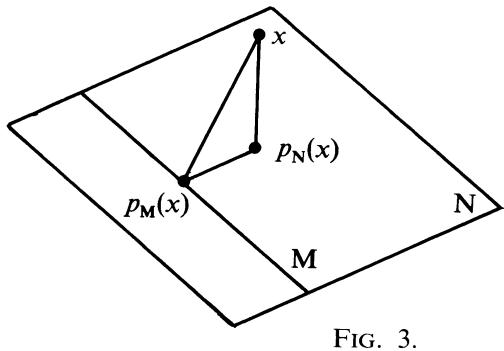
\includegraphics[keepaspectratio]{images/part002_dc4b20c6.jpg}}

